   
\section{Methodology}
\subsection{Data Imbalance}

The initial issue faced was how to split the continuous variables supplied by the EmoBank dataset into discrete categories.

An inital look at the data shows that there is a large number of sentences represented with valence values in the neutral, and very few representing the extreme cases. 

LINE GRAPH WITH NUMBER OF SAMPLES

The simplest way to initially categorise the data is to round to the nearest whole number, but as shown in figure \ref{dist:5cat}, the extreme classes are not well represented, and would prove very difficult to train a model off since there is such little data there to provide insight. Also having 5 discrete classes for each dimension provides more detail than is necessary for the task at hand.


\begin{figure}[h]
\caption{Graph showing data distribution when split into five classes}
\centering
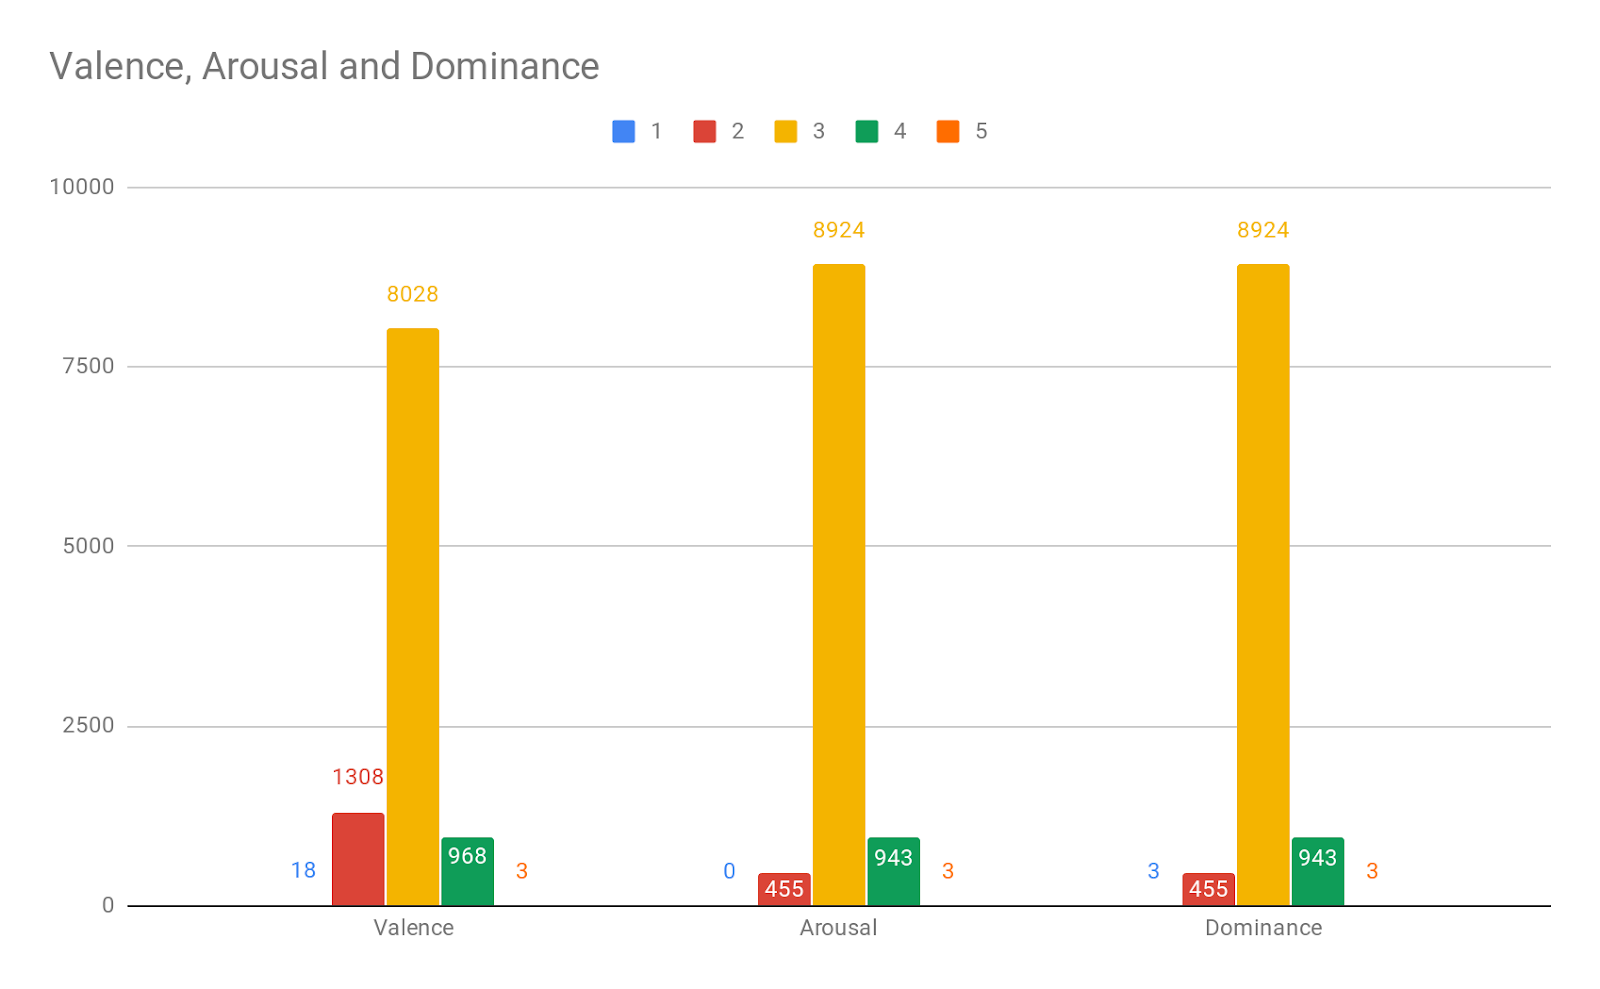
\includegraphics[scale=0.3]{graphs/5catDist.png}
\label{dist:5cat}
\end{figure}


Splitting each dimension up into positive or negative values, splitting each sentence into whether it is above or below 2.5 also is an option, allowing easier analysis to compare to other work which generally does just split the valence into positive or negative. The issue here is that the data imbalance is still very great, particularly with the Arousal and Dominance dimensions.

\begin{figure}[h]
\caption{Graph showing data distribution when split into binary positive and negative classes}
\centering
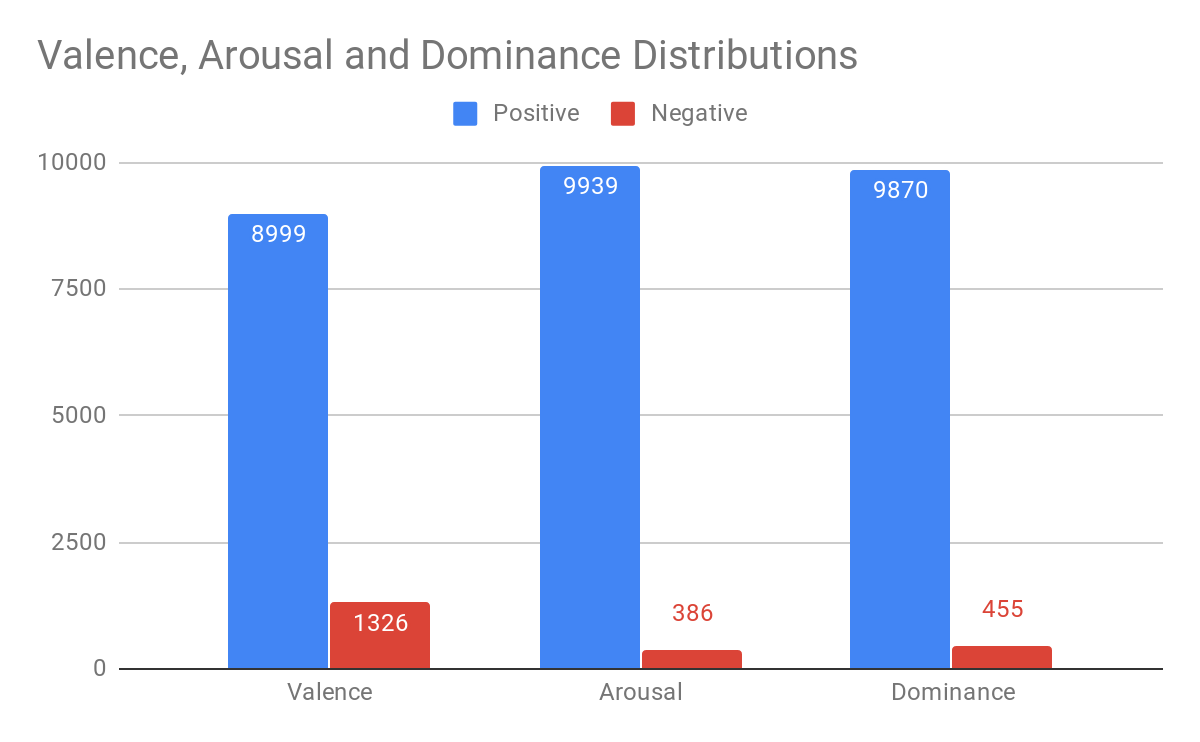
\includegraphics[scale=0.3]{graphs/binaryDist.png}
\end{figure}

A middle ground can be found when splitting the data into positive, neutral and negative classes, as even though there is still a data imbalance there, it is less severe, and so is used for the rest of analysis over the data.

\begin{figure}[h]
\caption{Graph showing data distribution when split into positive, neutral negative classes}
\centering
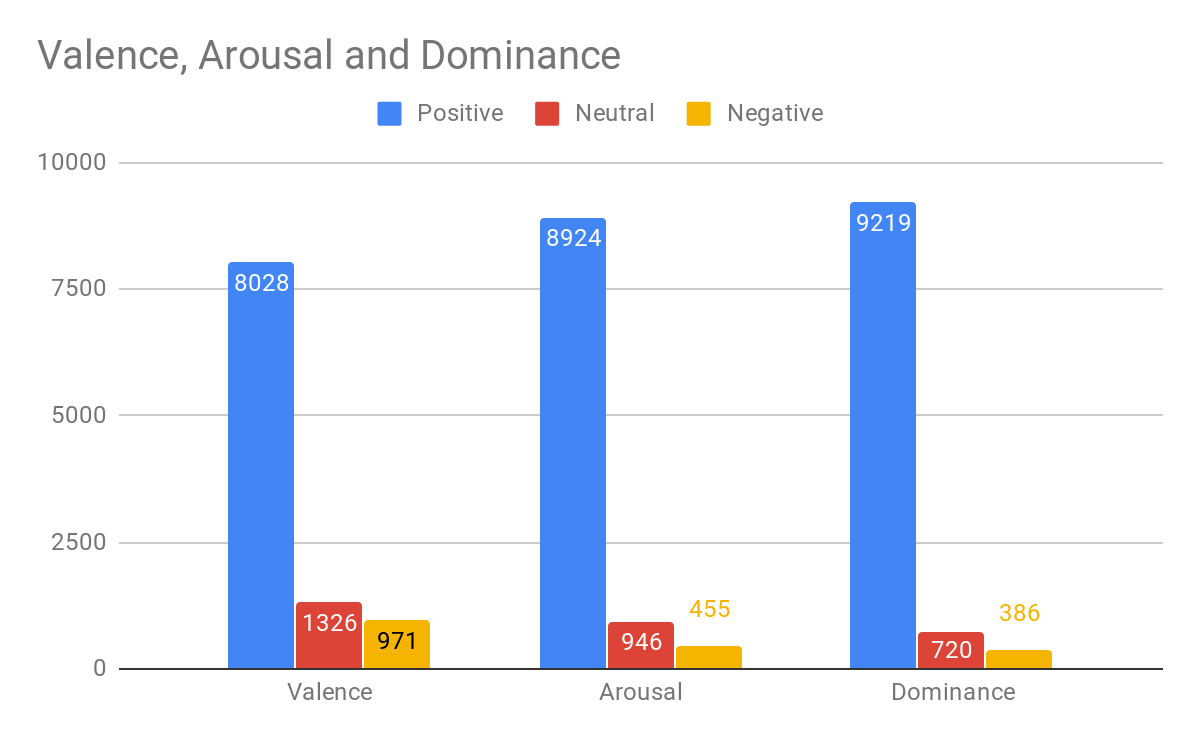
\includegraphics[scale=0.3]{graphs/nonBinaryDist.png}
\end{figure}



\subsection{Hypothesis Tests}


To argue for each of the decisions made when building the final model, a hypothesis test with a 95\% confidence level will be carried out.

Due to the imbalance in the data, a prediction accuracy cannot be used for comparing the models. This is because the majority class dominates, with it being the most likely to be predicted as there are simply more examples available. \cite{al2015applied} 

The F1 score of the prediction model is used in the hypothesis tests. The F1 score is the weighted average of the Precision and Recall of a model, which are defined as follows: 

$$ F1 = 2 * \frac{Precision * Recall}{Precision + Recall} $$

Precision is the ratio of correctly predicted positive observations to the total predicted positive observations.

$$ Precision = \frac{True Positive}{True Positive + False Positives} $$

Recall is the ratio of correctly predicted positive observations to the all observations in actual class. 

$$ Recall = \frac{True Positive}{True Positive + False Negatives} $$

For each investigation that is carried out, a confusion matrix will be produced so that the precision and recall values for each result can be calculated, which will have the following structure: 



\begin{center}
\begin{tabular}{ |p{3cm}|p{3cm}|p{3cm}|p{3cm}| }
 \hline
  & \multicolumn{3}{|c|}{Predicted} \\
 \hline
   Actual & Negative & Neutral & Positive\\
    \hline
    Negative &  True Negative   &  False Negative  & False Negative\\
    Neutral & False Neutral & True Neutral&  False Neutral \\
    Positive & False Positive & False Positive &  True Positive\\
 \hline
\end{tabular}

\end{center}
This will allow for the easy calculation of the F1 score for each investigation.


The hypothesis test that will be performed on the data will be the Wilcoxon Signed-Rank Test, since the comparison between the data will be on two related samples, looking for differences in their population rank means, and the data cannot be assumed to be normally distributed, meaning that this is the best test to be using in this case. \cite{wilcoxon1970critical}


Each of the experiments are run with k fold validation, with the data from each fold being used for test comparisons.


\subsection{Data Pre-processing (N-Gram and Feature selection)}


\begin{figure}[h]
\caption{ngram features}
\centering
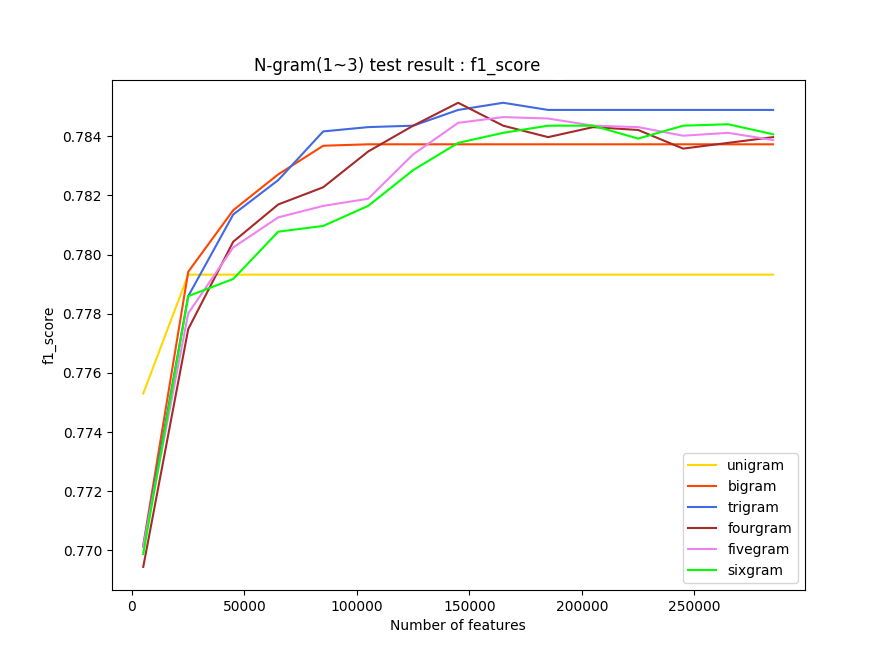
\includegraphics[scale=0.6]{graphs/ngramfeatures.png}
\end{figure}



\subsection{Model Selection}
\begin{itemize}
    \item Be critical, strengths and weaknesses of existing work
\end{itemize}


\begin{figure}[h]
\caption{models}
\centering
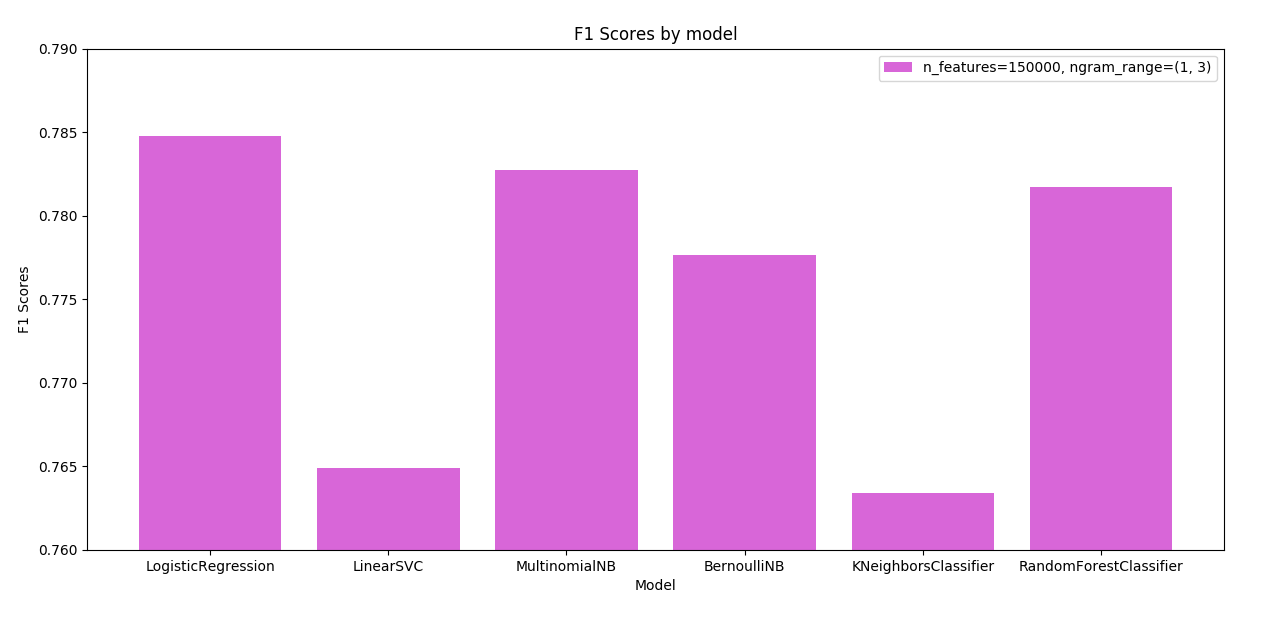
\includegraphics[scale=0.4]{graphs/models.png}
\end{figure}




\subsection{Oversampling and Undersampling}

\begin{figure}[h]
\caption{oversample}
\centering
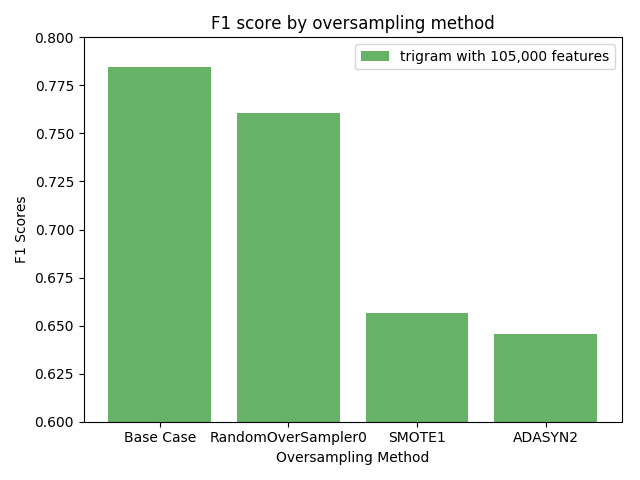
\includegraphics[scale=0.5]{graphs/oversampling.png}
\end{figure}


\begin{figure}[h]
\caption{undersample}
\centering
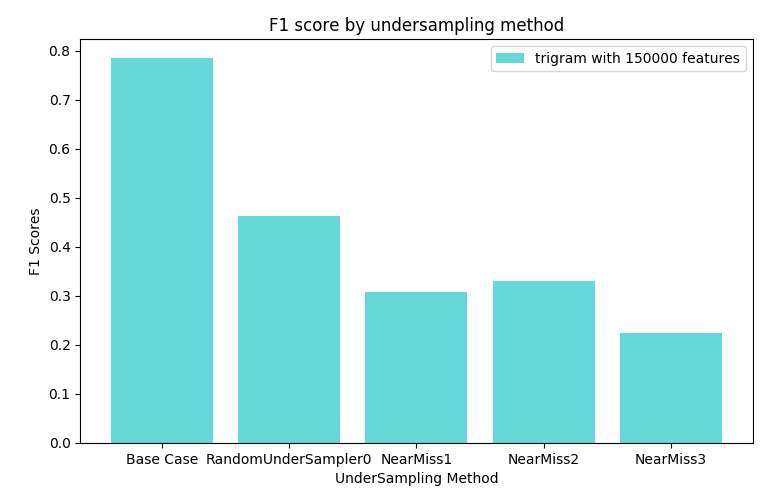
\includegraphics[scale=0.5]{graphs/undersample.png}
\end{figure}

\subsection{Implementation}